\documentclass[review]{elsarticle}
%\usepackage[utf8]{vietnam}
\setlength{\parskip}{10pt}
%\usepackage[pdftex]{graphicx}
%\usepackage[font=footnotesize]{caption}

\usepackage{mwe}    % loads »blindtext« and »graphicx«
\usepackage{subfig}
\usepackage{array}
\usepackage{float}
\usepackage{subfloat}
\usepackage{sidecap}
%\usepackage{caption}
\usepackage{epstopdf}
%\usepackage{subfigure}

\usepackage{mathtools}

\usepackage{graphics}

% %Packages used to make a confusion matrix
\usepackage{tabularx}
\usepackage{colortbl}
\usepackage{hhline}

\usepackage{lineno,hyperref}
\modulolinenumbers[5]

\journal{Journal of \LaTeX\ Templates}

\captionsetup[subfigure]{subrefformat=simple,labelformat=simple,listofformat=subsimple}
\renewcommand\thesubfigure{(\alph{subfigure})}

%%%%%%%%%%%%%%%%%%%%%%%
%% Elsevier bibliography styles
%%%%%%%%%%%%%%%%%%%%%%%
%% To change the style, put a % in front of the second line of the current style and
%% remove the % from the second line of the style you would like to use.
%%%%%%%%%%%%%%%%%%%%%%%

%% Numbered
%\bibliographystyle{model1-num-names}

%% Numbered without titles
%\bibliographystyle{model1a-num-names}

%% Harvard
%\bibliographystyle{model2-names.bst}\biboptions{authoryear}

%% Vancouver numbered
%\usepackage{numcompress}\bibliographystyle{model3-num-names}

%% Vancouver name/year
%\usepackage{numcompress}\bibliographystyle{model4-names}\biboptions{authoryear}

%% APA style
%\bibliographystyle{model5-names}\biboptions{authoryear}

%% AMA style
%\usepackage{numcompress}\bibliographystyle{model6-num-names}

%% `Elsevier LaTeX' style
\bibliographystyle{elsarticle-num}
%%%%%%%%%%%%%%%%%%%%%%%

\begin{document}

\begin{frontmatter}

\title{Pseudo-3D Trajectories: An Effective Approach for Motion Representation in Depth Data}

%% Group authors per affiliation:
\author{Chien-Quang LE}
\address{The Graduate University for Advanced Studies}

\author{Duy-Dinh LE}
\address{National Institute of Informatics, The Graduate University for Advanced Studies}

\author{Shin'ichi SATOH}
\address{National Institute of Informatics, The University of Tokyo}


\begin{abstract}
Leveraging the motion information of trajectories shows the effectiveness to the human action recognition in intensity videos. However, the issue is that this approach direction is effective or not when represents motions in depth video is not still answered. In this paper, we will deal with this issue by conducting experiments based on intensity trajectory features to present motion information from one depth video representation. Beside, in order to ensure including depth information, we propose a method based on compensating motion information from other representations. Evaluated on the benchmark datasets, our method significantly outperforms the state-of-the-art depth-based methods.
\end{abstract}

\begin{keyword}
\texttt{Trajectory, action recognition, depth data, feature representation}
%\MSC[2010] 00-01\sep  99-00
\end{keyword}

\end{frontmatter}

\linenumbers

\section{Introduction}

%\paragraph{Background and Challenges}
Recently, with the development of RGB-D cameras such as Kinect, depth data pioneers many potential research directions for human action recognition. Compared with conventional intensity images, depth maps support more several advantages. For example, depth maps provide shape information, which can be clearer than intensity images. Moreover, the depth data is less affected by illumination variations. However, an issue is that intensity-based methods are effective or not on depth data, which has not been much interested.

%\paragraph{Existing approaches and drawbacks} 
For action recognition, in order to effectively adapt intensity-based methods for depth data, we need satisfy two major factors. Firstly, a robust feature representation is extremely important to exactly capture motion information. Secondly, to ensure that a motion contains full information in depth video, merging depth information into feature representation is an indispensable requirement. However, the recent proposed methods do not combine two the factors completely. Works \cite{yang2012recognizing, xia2013spatio} consider depth value as intensity value and adapt the intensity-based techniques. Although, they can achieve reasonable results, they deal with many limitations. \cite{yang2012recognizing} can leverage depth information from the projections of depth maps. But its feature representation based on global motion such as HOG easily cause confusion by similar postures. \cite{xia2013spatio} can ensure depth information in feature descriptor computation. But this approach does not guarantee the reliability when extracting local points, due by textureless data and depth noise. Beside, methods in \cite{wang2012mining, oreifej2013hon4d} only focus on exploiting depth information without leveraging the effectiveness of the intensity-based features. Therefore, we propose an effective method that can satisfy both mentioned factors.

\begin{figure}
	\begin{center}
		\subfloat[From front view]{\label{subfig1:FrontView}
			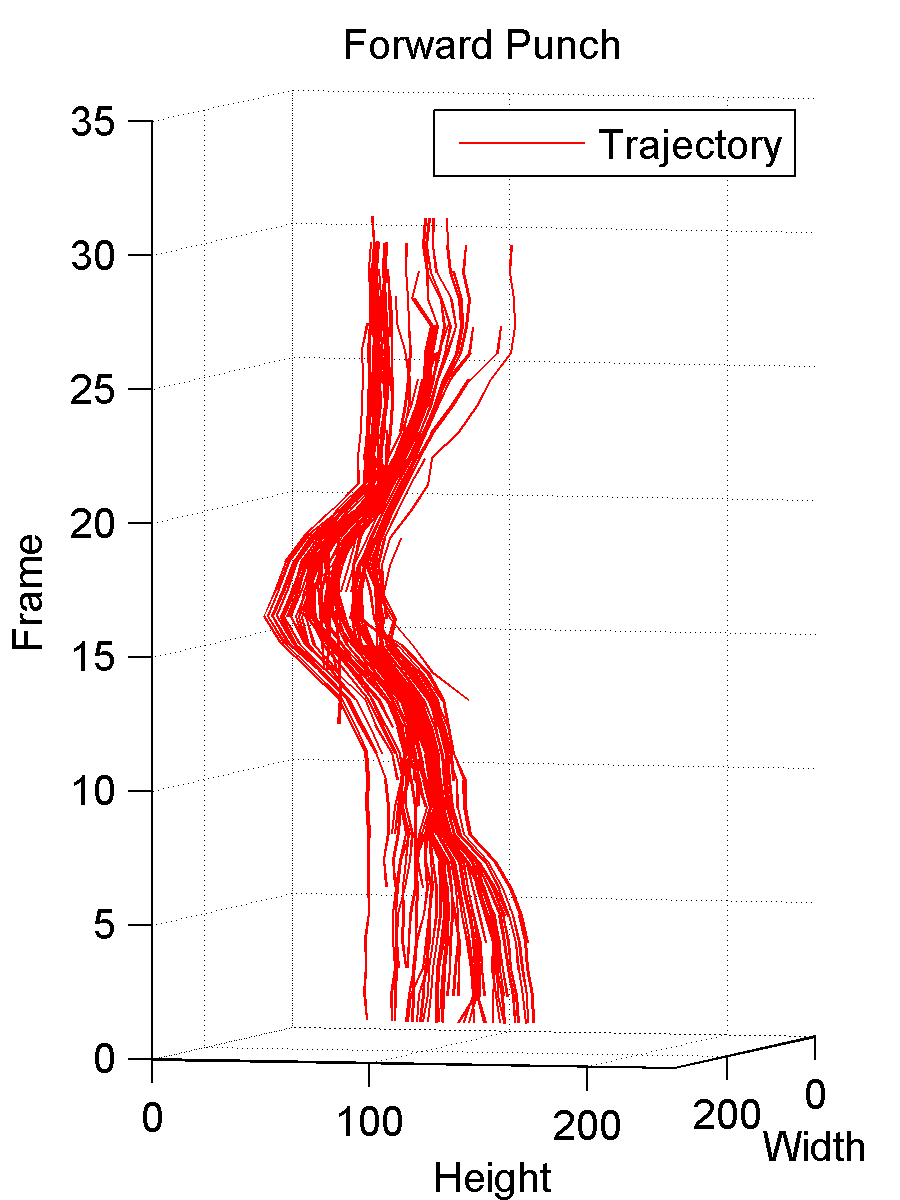
\includegraphics[scale=0.5]{ForwardPunch_FRONT.png}
			\hspace{2cm}
			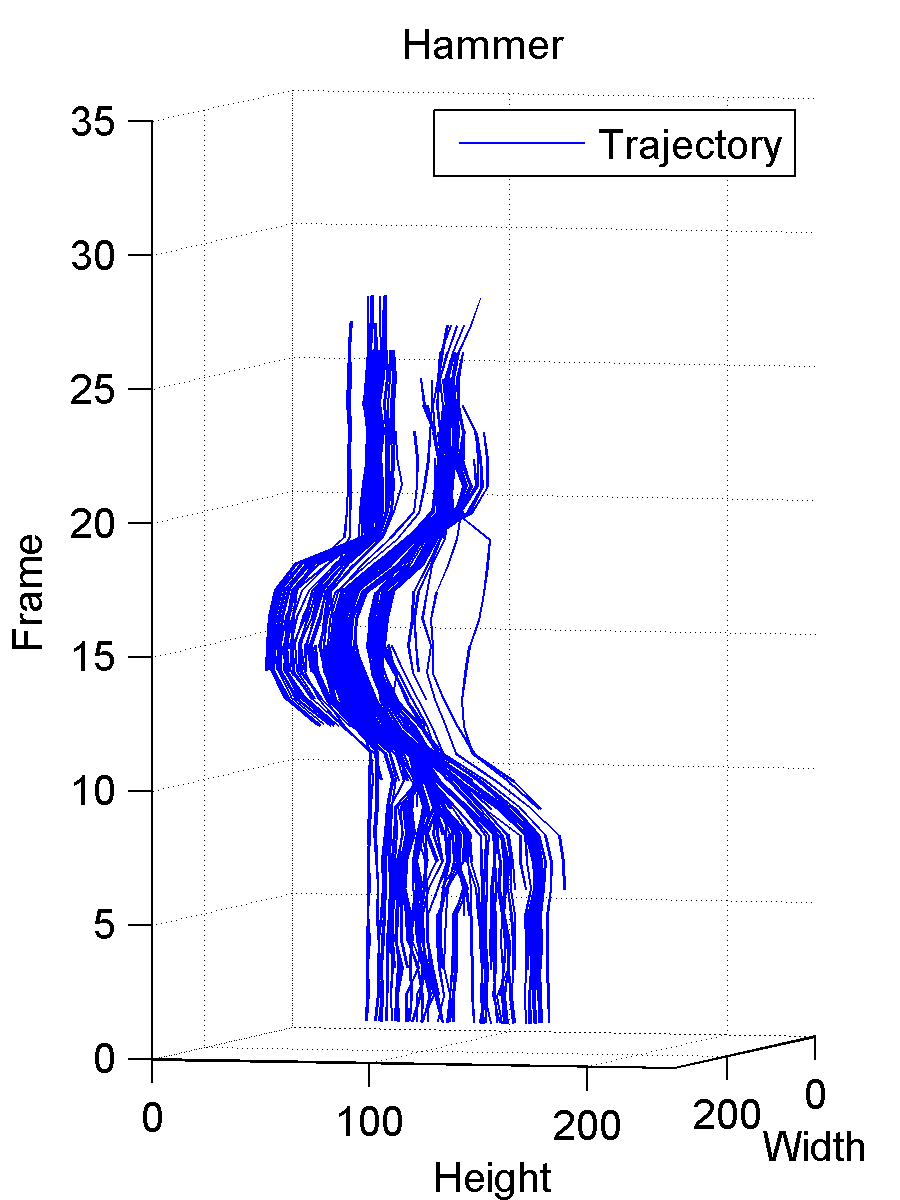
\includegraphics[scale=0.5]{Hammer_FRONT.png}
		}
	\end{center}
	\begin{center}
		\subfloat[From side view]{\label{subfig2:SideView}
			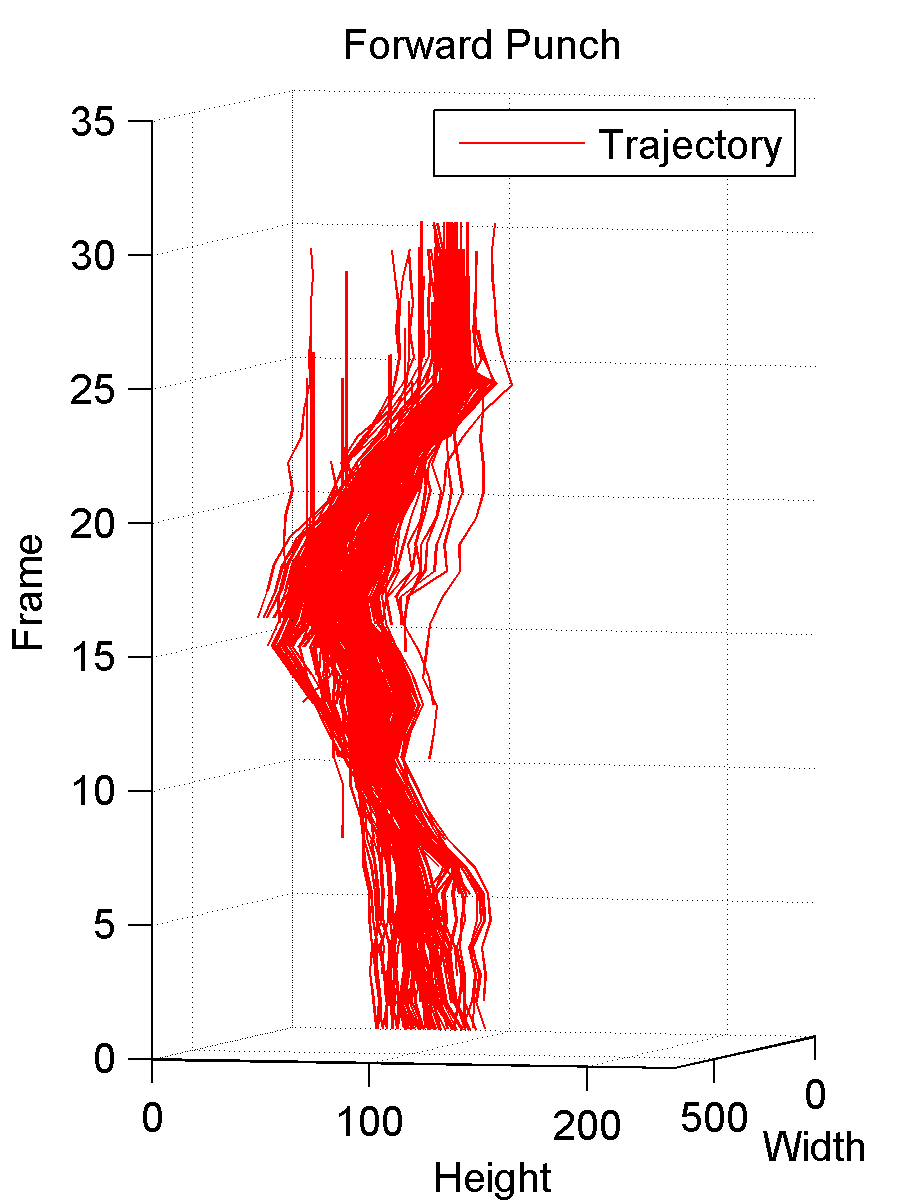
\includegraphics[scale=0.5]{ForwardPunch_SIDE.png}
			\hspace{2cm}
			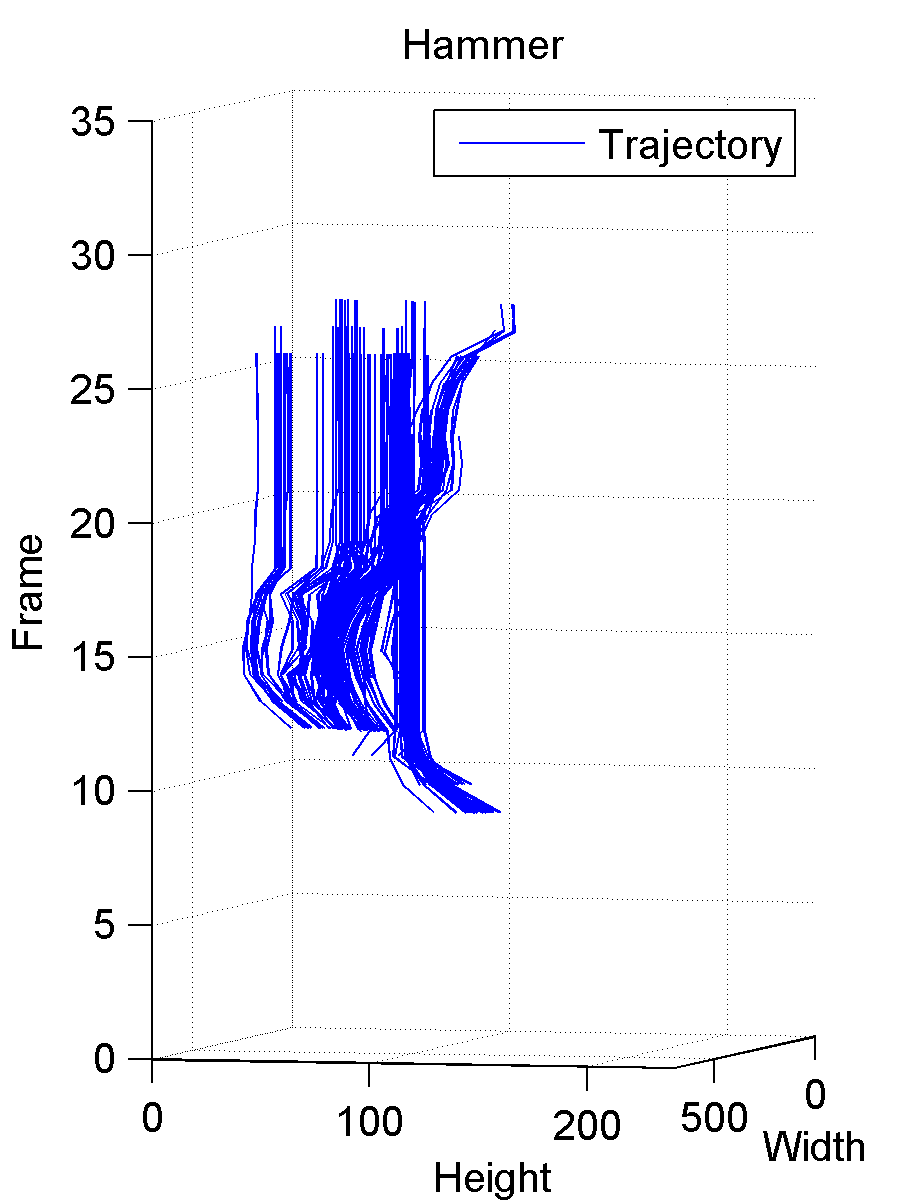
\includegraphics[scale=0.5]{Hammer_SIDE.png}
		}
	\end{center}
	\begin{center}
		\subfloat[From top view]{\label{subfig3:TopView}
			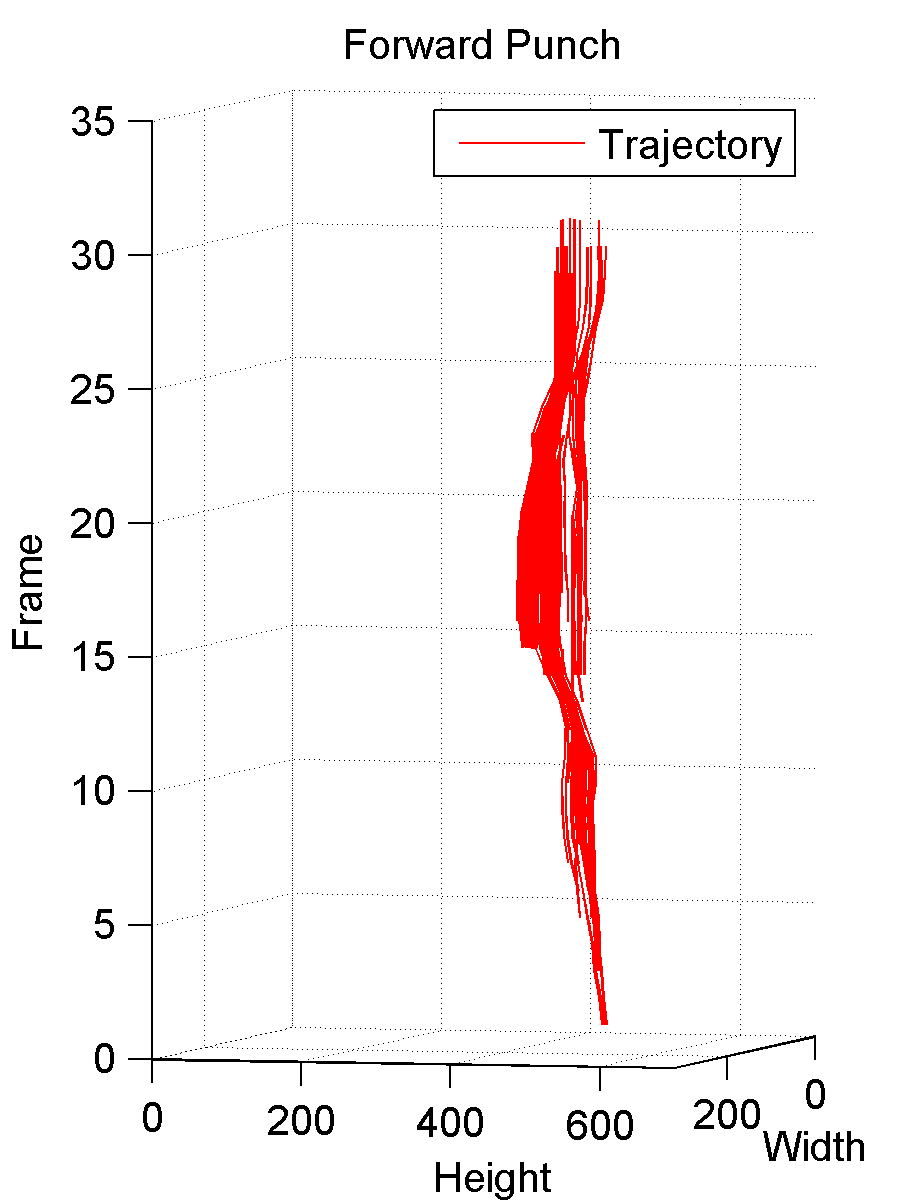
\includegraphics[scale=0.5]{ForwardPunch_TOP.png}
			\hspace{2cm}
			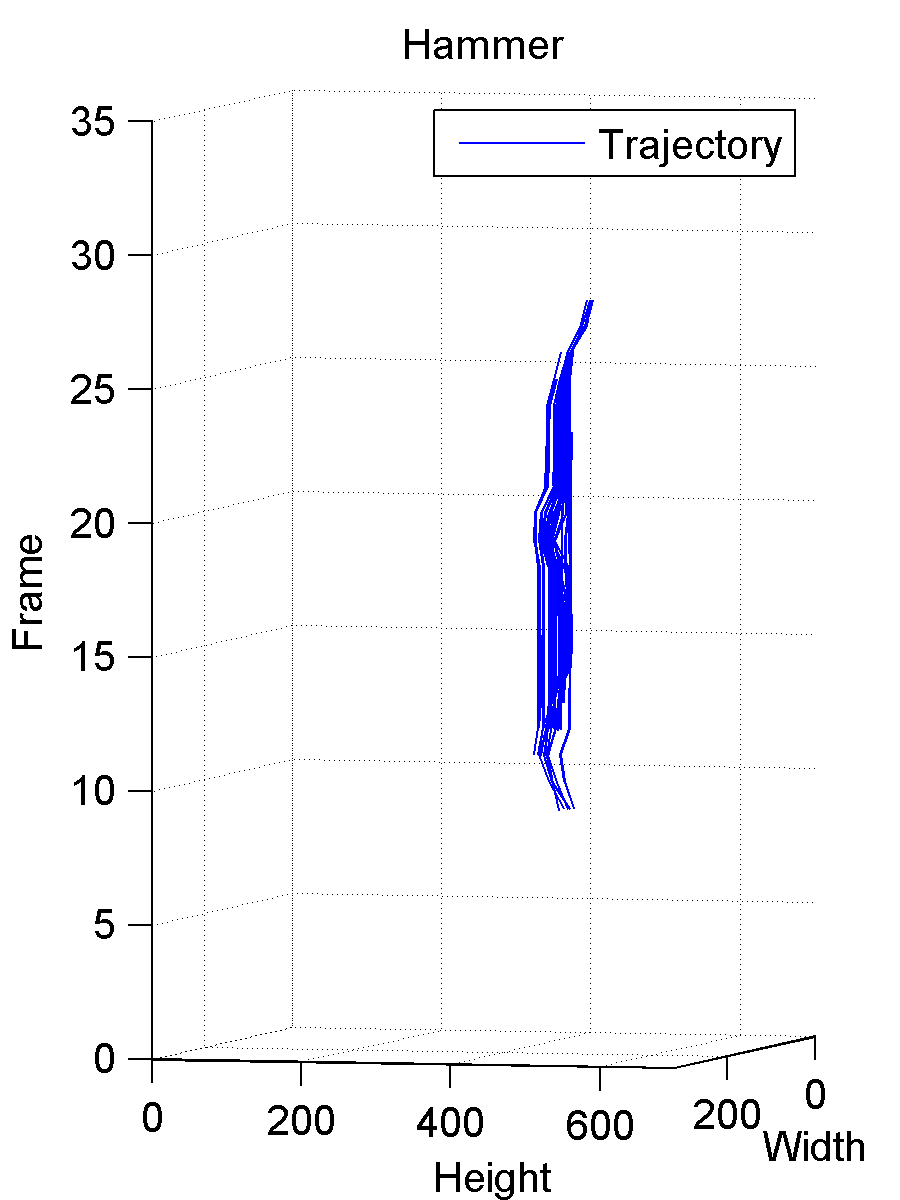
\includegraphics[scale=0.5]{Hammer_TOP.png}
		}
	\end{center}
	\caption{An illustrative comparison between trajectories' shape of actions \textit{Forward Punch} and \textit{Hammer}.}
	\label{fig:Illustration}
\end{figure}

%\paragraph{Proposal, Idea and Steps}
In this paper, we use a feature representation based on dense trajectories proposed by \cite{wang2011densetraj}, due to the effectiveness of this approach in many problems, including  activity recognition and multimedia event detection (MED). The trajectories obtained by tracking densely sampled points using optical flow fields. After extracting the trajectories, trajectory-aligned descriptors will be adopted. Then, features computed from the descriptors will be used to represent motion information in video.

However, the lack of depth information in feature representation can cause several confused cases, as shown in figure \ref{subfig1:FrontView}. Thus, to ensure that depth information is not ignored, a basic idea is to combine the motion information from various views. The view-based representations can be achieved by projecting depth maps onto the corresponding planes. The projections are easily obtained by the mentioned advantages of depth data.

%\paragraph{Experiments and Results}
We conduct experiments on MSR Action 3D dataset and MSR Daily Activity 3D dataset. Experimental results show that our proposed method beats the state-of-the-art methods in constrain of only using depth data. The results also present our contributions: (1) We propose an adaptive method for depth video representation by using intensity-based features. (2) We perform comprehensive experiments on the challenging benchmark datasets and indicate that our method is the best when compared with the state-of-the-art depth-based methods.

%\paragraph{Paper structure}
After a brief review of the related work in Section \ref{lbl:RelatedWorks}, the proposed method is described in Section \ref{lbl:ProposedMethod}. Sections \ref{lbl:ExperimentalSettings} and \ref{lbl:ExperimentalResults} present the experimental settings and results. In section \ref{lbl:Discussions} we provide some concerned discussions. The summaries of our work are given in Section \ref{lbl:Conclusions}.

% % Vietnamese version
%\paragraph{Background and Challenges} Gần đây, với sự phát triển của RGB-D camera như Kinect, depth data đã mở ra nhiều hướng nghiên cứu tiềm năng cho bài toán Human Action Recognition. So sánh với intensity images thông thường, depth maps hỗ trợ nhiều advantages hơn. Ví dụ, depth maps cung cấp các thông tin về shape rõ ràng hơn so với intensity images. Hơn thế nữa, depth data ít bị ảnh hưởng bởi những thay đổi của ánh sáng. Tuy nhiên, các phương pháp dựa trên intensity liệu có hiệu quả trên depth data hay không vẫn chưa được quan tâm nhiều.

%\paragraph{Existing approaches and drawbacks} Trong bài toán action recognition, để adapt các phương pháp dựa trên intensity cho depth data có 2 yếu tố chính. Thứ nhất, để capture motion information hiệu quả việc chọn lựa a robust feature representation là rất quan trọng. Thứ hai, để đảm bảo motion là đầy đủ thông tin trong depth video, việc bổ sung thông tin depth vào feature representation là yêu cầu không thể thiếu. Tuy nhiên, các phương pháp được đề xuất gần đây vẫn chưa hội tụ đủ 2 yếu tố này. Một số phương pháp như \cite{yang2012recognizing, xia2013spatio} xem xét depth value như là intensity value và adapt các intensity-based techniques. Mặc dù, chúng có thể đạt được những kết quả hợp lý, nhưng tất cả chúng đều phải đối mặt với nhiều hạn chế. [DMM-HOG] có thể tận dụng thông tin depth từ các phép chiếu của depth maps. Nhưng its feature representation dựa trên global motion như HOG sẽ dễ gây nhầm lẫn bởi những similar postures. \cite{xia2013spatio} có thể đảm bảo depth information trong việc tính toán features. Nhưng cách tiếp cận này không đảm bảo được sự tin cậy khi extract các local points, do bởi textureless data and depth noise. Ngoài hướng tiếp cận trên, các phương pháp như \cite{wang2012mining, oreifej2013hon4d} chỉ tập trung khai thác depth information nên không tận dụng được sức mạnh của các intensity-based features. Do đó, hướng nghiên cứu của chúng tôi là propose một phương pháp có thể đáp ứng đầy đủ cả 2 yếu tố nêu trên.

%\paragraph{Proposal, Idea and Steps}Trong bài báo này, chúng tôi sử dụng một feature representation dựa trên dense trajectories của \cite{wang2011densetraj}, do bởi hiệu quả của cách tiếp cận này trong nhiều bài toán, including activity recognition and multimedia event detection. Các trajectories thu được bằng cách tracking các sampled points densely sử dụng optical flow fields. Sau khi extract trajectories, các trajectory-aligned descriptors sẽ được adopted. Sau đó, features tính toán được từ các descriptors này sẽ được sử dụng cho việc biểu diễn motion information trong video.

%Tuy nhiên, việc thiếu sót depth information trong feature representation có thể gây ra các trường hợp bị confused, như được chỉ ra trong Figure \ref{subfig-1:FrontView}. Do đó, để đảm bảo việc không bỏ sót thông tin depth, ý tưởng cơ bản là combine thông tin chuyển động từ nhiều góc nhìn khác nhau. Các biểu diễn từ nhiều góc nhìn có thể đạt được bằng cách chiếu depth maps lên trên các mặt phẳng tương ứng. Việc chiếu này dễ dàng thực hiện được bởi những thuận lợi mà depth data mang lại.

\section{Related Works}
\label{lbl:RelatedWorks}

\subsection{Trajectories Extraction}
Trajectories provide a compact representation of motion information in video. Trajectories from intensity videos can be used for multimedia event detection (MED), video mining, action classification and so on. Trajectory extraction much depends on both processes: sampling and tracking. Some concerned methods, such as \cite{matikainen2009trajectons, messing2009activity} used KLT tracker \cite{lucas1981iterative}, or \cite{sun2009hierarchical} matched  SIFT descriptors between consecutive frames to obtain feature trajectories. Recently, the dense trajectories feature proposed by \cite{wang2011densetraj} has achieved state-of-the-art performances on MED systems, such as, segment-based system \cite{phan2014multimedia} on TRECVID MED 2010, 2011, or AXES \cite{oneata2012axes}, and BBNVISER \cite{natarajan2012bbn} on TRECVID MED 2012.

Although, depth data has been studied ago several decades, the trajectory extraction in depth videos is not still paid attention to. This is obviously a significant deficiency for motion-based recognition systems using depth data.

\subsection{Feature Representation from Depth Videos}
In terms of human action recognition in depth video, most recent methods exploit depth information into two major directions. The first one is adapting intensity techniques-based methods for depth data. The second one is to use depth value as its mean.

For the first direction, Yang.X et al. \cite{yang2012recognizing} propose the Depth Motion Maps (DMM) to accumulate global activities in depth video sequences. And the Histogram of Oriented Gradients (HOG) are computed from the DMM to represent an action video. Another approach bases on spatio-temporal interest points proposed by Xia.L and Aggarwal.J.K \cite{xia2013spatio}. In this approach, they extend a work of Dollar et al. \cite{dollar2005behavior} to adapt for depth data.

For the second direction, \cite{li2010action} uses a bag of 3D points to characterize a set of salient postures. The 3D points are extracted on the contours of the planar projections of the 3D depth map. And then, about 1\% 3D points are sampled to calculate feature. \cite{vieira2012stop, wang2012robust, wang2012mining} use occupancy patterns to represent feature in action video. Another approach proposed by Oreifej et al. \cite{oreifej2013hon4d} leverages the distribution of surface normal orientation in the 4D space of time, depth and spatial coordinates to build a feature histogram. Inspired by results of Shotton et al. \cite{shotton2013real} and Xia.L et al. \cite{xia2011human}, works \cite{yang2012eigenjoints, wang2012mining} propose new types of features based on skeleton information.

Different from other approaches, we use a trajectory-based approach for action recognition. We do not care to segment human body like \cite{li2010action,yang2012recognizing}. We only investigate the benefit of generating intensity representations from depth data, as mentioned in \cite{li2010action,yang2012recognizing}. Moreover, we leverage the effectiveness of trajectory feature to represent an action video. In our best knowledge, no method has previously proposed adapting trajectory-based approach for human action recognition in depth video. We conduct evaluations on recognition accuracy using dense trajectories motion feature proposed by Wang et al. \cite{wang2011densetraj}.

\section{Proposed Method}
\label{lbl:ProposedMethod}

This paper presents a effective depth video representation by adapting intensity trajectories-based motion features. First, we provide a brief review of the dense trajectories-based feature proposed by Heng Wang et al. \cite{wang2011densetraj}. Related parts, such as: dense sampling, tracking and feature descriptors are also referred to. Our trajectories-based approach for depth data is mentioned at the end of this section.

\subsection{Dense trajectories}
% - Giới thiệu khái quát về dense trajectories
In order to obtain trajectories, there are two important steps: sampling and tracking. \cite{wang2011densetraj} propose sampling on a dense grid with a step size of 5 pixels. The sampling is performed at multiple scales with a factor of $1/\sqrt{2}$. Then, tracking is the next step to form trajectories. At each scale, in frame \textit{t}, each point \textit{$P_t = (x_t, y_t)$} is tracked to point \textit{$P_{t+1} = (x_{t+1}, y_{t+1})$} in next frame \textit{t+1} by:
\begin{equation}
	\textit{$P_{t+1} = (x_{t+1}, y_{t+1}) = (x_t, y_t) + (M*\omega)|_{(\bar{x}_t,\bar{y}_t)} $},
\end{equation}
where \textit{$\omega = (u_t, v_t)$} denotes the dense optical flow field, \textit{M} is the kernel of median filtering, and \textit{$(\bar{x}_t,\bar{y}_t)$} is the rounded position of \textit{$P_t$}. The algorithm of \cite{farneback2003two} is adopted to compute the dense optical flow. And to avoid a drifting problem, a suitable value of trajectory length is set to 15 frames. Beside, trajectories with sudden changes are removed.

After extracting trajectories, two kinds of descriptors: a trajectory shape descriptor and a trajectory-aligned descriptor can be adopted.

\paragraph{Trajectory Shape Descriptor}This descriptor describes the shape of a trajectory in the simplest way. Given a trajectory of length L, its shape is concatenated by a sequence of displacement vectors \textit{$S = (\Delta P_t, ..., \Delta P_{t+L-1})$}, where \textit{$\Delta P_t = P_{t+1} - P_t = (x_{t+1} - x_t, y_{t+1} - y_t)$}. In order to make the descriptor invariant to scale changes, the final result is then achieved by normalizing the shape vector by the overall magnitude of the displacement vectors:

\begin{equation}
	\textit{$\bar{S} = \frac{(\Delta P_t, ..., \Delta P_{t+L-1})}{\sum_{k=t}^{t+L-1}\|\Delta P_k\|}$},
\end{equation}

\paragraph{Trajectory-aligned Descriptor}The descriptors are much more complex than the trajectory shape descriptor. They are computed within a space-time volume ($N \times N$ spatial pixels and $L$ temporal frames) around the trajectory. This volume is divided into a 3D grid (spatially $n_\sigma \times n_\sigma$ grid and temporally $n_\tau$ segments). The default settings of these parameters are $N$ = 32 pixels, $L$ = 15 frames, $n_\sigma$ = 2, and $n_\tau$ = 3.

In order to capture the local motion and appearance around a trajectory, three kinds of descriptors have been employed: the Histogram of Oriented Gradient (HOG) \cite{dalal2005histograms}, the Histogram of Optical Flow (HOF) \cite{laptev2008learning}, and the Motion Boundary Histogram (MBH) \cite{dalal2006human}. For HOG, orientation information is quantized into 8-bin histogram. HOF is 9-bin histogram. Since the feature of a trajectory is calculated and concatenated from sub-volumes of a 3D volume, the final representation has 96 dimensions for HOG and 108 dimensions for HOF. MBH descriptor computes derivatives on both horizontal and vertical components of optical flow $I_\omega = (I_x. I_y)$. Similar to HOG descriptor, the orientation information is quantized into 8-bin histogram. Since the motion information is combined along two directions, the final representation is $96 \times 2 = 192$-bin histogram. By presenting gradient of optical flow, MBH descriptor is able to suppress global motion information and only keep local relative changes in pixels.

According to the authors \cite{laptev2008learning, wang2011densetraj, wang2009evaluation, liu2009recognizing}, all the three descriptors have shown the effectiveness for action recognition. The experimental settings for these descriptors are based on an empirical study showed in \cite{wang2011densetraj}. We also conduct our experiment on all the three descriptors when compared to the depth-based state-of-the-art methods.

\subsection{Pseudo-3D trajectory-based Approach for Motion Feature in Depth Data}

Our proposed trajectory-based approach for human action recognition in depth data is as follow. At first, intensity representations are formed from the sequence of depth maps, as illustrated in Figure \ref{lbl:Figure_ProposedMethod}. In particular, we choose three representations to represents for 3 view directions: front, side, and top in 3D space. Forming the representations is necessary due to dimensional gap when we adapt 2D techniques for 3D data. After that, the dense trajectories are extracted from the intensity representations. And the feature descriptors are also computed in this step. At the next step, with each intensity representation, corresponding feature representation is quantized from raw trajectory features by apply a bag-of-words (BoW) model. An \textit{early fusion} scheme is used to generate the final feature representation for action in the sequence of depth maps (Fig. \ref{lbl:Figure_Framework}).

\begin{figure}[H]
	\begin{center}
		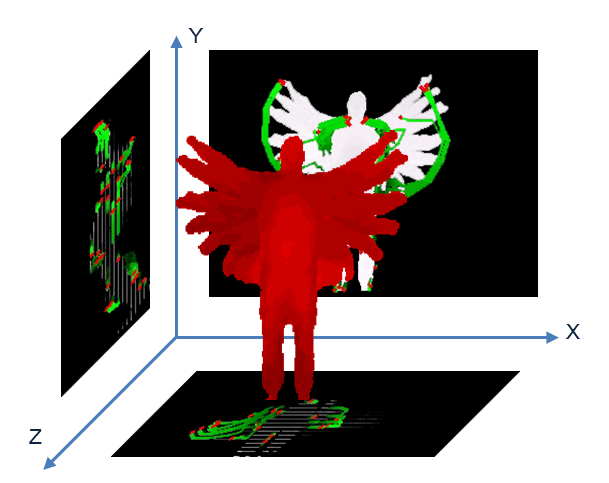
\includegraphics[width=0.7\textwidth]{Projections.png}
	\end{center}
	\caption{\label{lbl:Figure_ProposedMethod}Illustration of our trajectory-based approach. The original sequence of depth maps is projected onto three orthogonal planes to form intensity videos. After that, the dense trajectory motion features are calculated for each representation.}
\end{figure}

%- Hình 2 - Illustration of proposed method - Depth maps -> 3 projections -> dense trajectories

In order to generate intensity representations from the sequence of depth maps, we use the approach proposed in \cite{li2010action}. This technique is also used in \cite{yang2012recognizing}. Basically, this method projects depth maps onto three orthogonal planes in Casterian space to obtain corresponding intensity representations. However, motion representation for human action in the previous approaches is accumulated from global motion information. Therefore, these approaches must deal with the challenges from human segmentation problem in more complicated datasets. In contrast to the previous ones, we pay attention to capture local motion information for representing human actions. With the approach, we do not care the challenges for segmenting human body. To effectively use local motion information, we leverage the effectiveness of trajectory-based representation. In practice, we adopt the dense trajectory-based approach proposed in \cite{wang2011densetraj}. Thus, motion information in depth data can be reproduced by complementary motion information in different intensity representations.

\begin{figure}[H]
%	\begin{center}
	\centering
%	\resizebox{1.2\textwidth}{!}{ %
		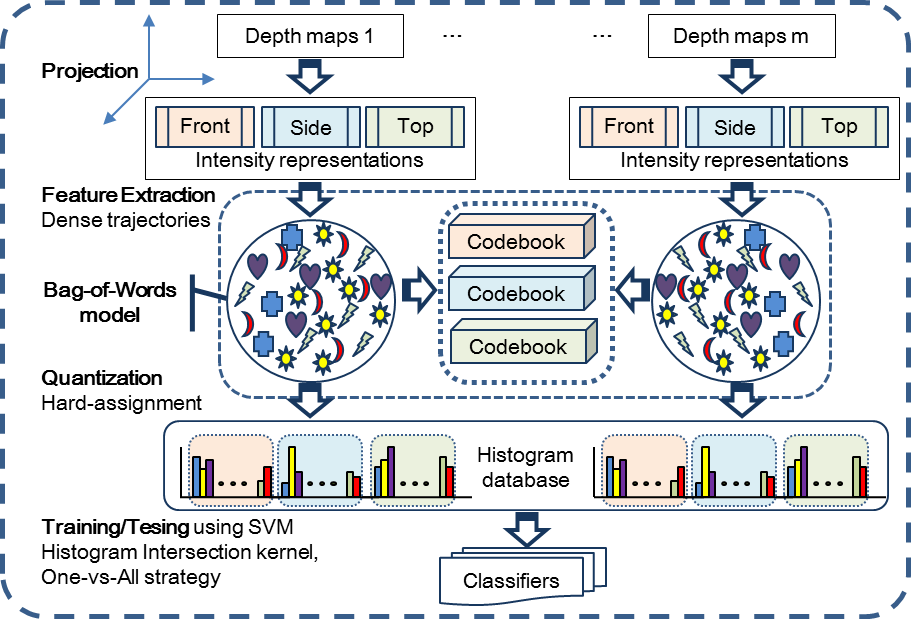
\includegraphics[width=\textwidth]{Framework3D.png} %
%	}
%	\end{center}
	\caption{\label{lbl:Figure_Framework}Our Framework Overview}
\end{figure}
%- Hình 3 - Framework overview for our system - Depth data -> 3 feature extraction -> 3 BoW model -> 3 histogramintersection-SVM -> concatenated-score features -> chi-kernel SVM classifier

Our proposed trajectory-based approach is compared with the state-of-the-art methods in human action recognition using depth data. Actually, our approach does not care skeleton extraction, which is used as an important factor in some works, such as \cite{wang2012mining, yang2012eigenjoints}. In fact, extracting skeleton exactly is still an unsolved problem, due to the challenges, such as cluttered background, hardware quality, camera motion, so on.

\section{Experimental Settings}
\label{lbl:ExperimentalSettings}

\subsection{Dataset}
We test our method on MSR Action 3D dataset. This dataset contains 20 actions, as showed in Table \ref{lbl:20actions}. Actions are performed by ten subjects for two or three times in the context of game console interaction. In total, there are 567 sequences of depth maps. The depth maps are shot at frame rate of 15 fps. The size of the depth map is $640 \times 480$, we resize into $320 \times 240$ to ensure processing efficiency.

\begin{table}[H]
	\begin{center}
		% Table generated by Excel2LaTeX from sheet 'MSRAction3D names'
		\begin{tabular}{c|c|c|c}
		
		  {\bf   ID  } & {\bf Action Name} &   {\bf   ID  } & {\bf Action Name} \\
		\hline
		             1 &  high arm wave &             11 &  two hand wave \\
		
		             2 & horizontal arm wave &             12 &    side-boxing \\
		
		             3 &         hammer &             13 &           bend \\
		
		             4 &     hand catch &             14 &   forward kick \\
		
		             5 &  forward punch &             15 &      side kick \\
		
		             6 &     high throw &             16 &        jogging \\
		
		             7 &         draw x &             17 &   tennis swing \\
		
		             8 &      draw tick &             18 &   tennis serve \\
		
		             9 &    draw circle &             19 &     golf swing \\
		
		            10 &      hand clap &             20 & pick up \& throw \\
		
		\end{tabular}
	\end{center}
	\caption{\label{lbl:20actions}20 actions in MSR Action 3D dataset}
\end{table}

In order to conduct a fair comparison, we use the same experimental settings as \cite{li2010action, yang2012eigenjoints, yang2012recognizing, wang2012mining, xia2013spatio, oreifej2013hon4d}. In the settings, the dataset is divided into three action subsets. Each subset has 8 actions (Table \ref{lbl:3ActionSubsets}). The two subsets AS1 and AS2 present that grouped actions have similar movements. The subset AS3 groups complex actions together. For instance, action \textit{hammer} seems to be confused with action \textit{forward punch} in AS1 or similar movements between action \textit{hand catch} and action \textit{side boxing} in AS2. As for each subset, we select half of the subjects as training and the rest as testing (i.e. cross subject test).

\begin{table}
	\begin{center}
		% Table generated by Excel2LaTeX from sheet 'Sheet3'
		\begin{tabular}{c|c|c}
		
		{\bf Action Subset 1} & {\bf Action Subset 2} & {\bf Action Subset 3} \\
		{\bf(AS1)} & {\bf(AS2)} & {\bf(AS3)} \\
		\hline
		horizontal arm wave &  high arm wave &     high throw \\
		
		        hammer &     hand catch &   forward kick \\
		
		 forward punch &         draw x &      side kick \\
		
		    high throw &      draw tick &        jogging \\
		
		     hand clap &    draw circle &   tennis swing \\
		
		          bend &  two hand wave &   tennis serve \\
		
		  tennis serve &    side-boxing &     golf swing \\
		
		pick up \& throw &   forward kick & pick up \& throw \\
		
		\end{tabular}
	\end{center}
	\caption{\label{lbl:3ActionSubsets}The three action subsets used in the experiments}
\end{table}

\subsection{Evaluation Method}


Figure 3 shows our evaluation framework for the trajectory-based features. We perform experiments using the proposed approach and compare with the state-of-the-art methods on depth data. We use the application available online\footnote{http://lear.inrialpes.fr/$\sim$wang/dense\_trajectories} to extract dense trajectories and aligned-features. To quantize a large number of features obtained by densely sampling, the BoW model is applied. At first, in each intensity representation, we randomly get about 80,000 extracted trajectories for clustering with K-mean algorithm. Then, a codebook of 2000 visual codewords is formed for each. After that, the hard-assignment technique is used to compute histograms of the visual words on the corresponding intensity representations.

Once all the BoW histograms are generated, we adopt the late-fusion scheme with the popular Support Vector Machine (SVM) for classification. In practice, we use the precomputed-kernel technique with the histogram intersection measurement for the classification step. In our implementation, we use the libSVM library published online by author\footnote{http://www.csie.ntu.edu.tw/$\sim$cjlin/libsvm/} and perform the one-vs-all strategy for multi-class classification. We adopt the format requirements of the library to synchronize the annotation and the data. For testing, the BoW histograms of corresponding intensity representations are concatenated to generate the final feature representation. The predicted value is defined as the maximum score obtained from all the classifiers. This score shows that a human action is confused with another or not.

\section{Experimental Results}
\label{lbl:ExperimentalResults}
This section presents the experimental results from applying our proposed approach on MSR Action 3D dataset. We also report the results on the main intensity representation (i.e. front projection). Beside, an evaluation related to selecting compensation information from other representations will be also mentioned. All the results are compared in terms of the accuracy. The best performance is highlighted in bold.

\subsection{Recognize Actions from An Intensity Representation}

Table \ref{lbl:Table_MBHvsSoAonFront} - lists the results from our trajectory-based approach on front representation. Interestingly, the result table indicates that this approach beats all the state-of-the-art methods based on silhouette features \cite{li2010action, yang2012recognizing}, skeletal joint features \cite{yang2012eigenjoints, wang2012mining}, local occupancy patterns \cite{wang2012robust, vieira2012stop}, normal orientation features \cite{oreifej2013hon4d} and cuboid similarity features \cite{xia2013spatio}. However, the results also show that there is significant difference of the performance among the used feature descriptors.

\begin{table}[H]
	\begin{center}
		% Table generated by Excel2LaTeX from sheet 'Methods'
		\begin{tabular}{c|c}
		
		  {\bf Method} & {\bf Accuracy (\%)} \\
		\hline
		Bag of 3D Points \cite{li2010action} &         74.70  \\
		
		      STOP \cite{vieira2012stop} &         84.80  \\
		
		EigenJoints \cite{yang2012eigenjoints} &         82.33  \\
		
		Random Occupancy Patterns \cite{wang2012robust} &         86.50  \\
		
		Local Occupancy Patterns \cite{wang2012mining} &         88.20  \\
		
		Depth Motion Maps-based HOG \cite{yang2012recognizing} &         91.63  \\
		
		Histogram of Oriented 4D Normals \cite{oreifej2013hon4d} &         88.89  \\
		
		Depth Cuboid Similarity Feature \cite{xia2013spatio} &         89.30  \\
		\hline
		    {\bf Ours} &   {\bf 94.53 } \\
		
		\end{tabular}  
	\end{center}
	\caption{\label{lbl:Table_MBHvsSoAonFront}Results on front representation using MBH descriptor.}
\end{table}

\begin{table}[H]
	\begin{center}
		% Table generated by Excel2LaTeX from sheet 'VIEWS_LateFusion'
		\begin{tabular}{ccc}
		
		       \multicolumn{ 3}{c}{{\bf Action Subsets}} \\
		\hline
		     {\bf AS1} &      {\bf AS2} &      {\bf AS3} \\
		\hline
		        92.45  &         92.04  &         99.11  \\
		
		\end{tabular}
	\end{center}
	\caption{\label{lbl:MBHandAS123}Results on three action subsets.}
\end{table}

Consider the results on action subsets reported in Table \ref{lbl:MBHandAS123}, we found that two	 subsets AS1, AS2 contain many confused actions. For example, action-pair \textit{hammer} and \textit{forward punch} in AS1, or \textit{side-boxing} and \textit{hand catch} in AS2, as showed in Table \ref{lbl:AS123ConfusionMatrix}. When analyzing confused actions, we found that the main cause is due to similar movements. And, since depth data is textureless, it makes recognition more difficult. That is a reason why we need compensate information from other intensity representations.
\begin{table}[H]
	\begin{center}
		\subfloat[Action Subset 1 \label{lbl:ConfMatAS1}]{ %
		\resizebox{0.9\textwidth}{!}{ %
			% Table generated by Excel2LaTeX from sheet 'Experiment-MSRDaily3D'
			\begin{tabularx}{\textwidth}{c|c|c|c|c|c|c|c|c|}
					\multicolumn{1}{c}{~}& \multicolumn{1}{c}{\bf a02} & \multicolumn{1}{c}{\bf a03} & \multicolumn{1}{c}{\bf a05} & \multicolumn{1}{c}{\bf a06} & \multicolumn{1}{c}{\bf a10} & \multicolumn{1}{c}{\bf a13} & \multicolumn{1}{c}{\bf a18} & \multicolumn{1}{c}{\bf a20} \\
				\hhline{~--------}
					{\bf a02} & \color{white}{\bf 0.83}\cellcolor[gray]{.2} & 0 & {\bf 0.17}\cellcolor[gray]{.8} & 0 & 0 & 0 & 0 & 0 \\
				\hhline{~--------}
					{\bf a03} & 0 & \color{white}{\bf 0.92}\cellcolor[gray]{.1} & {\bf 0.08}\cellcolor[gray]{.9} & 0 & 0 & 0 & 0 & 0 \\
				\hhline{~--------}
					{\bf a05} & 0 & {\bf 0.36}\cellcolor[gray]{.6} & \color{white}{\bf 0.64}\cellcolor[gray]{.4} & 0 & 0 & 0 & 0 & 0 \\
				\hhline{~--------}
					{\bf a06} & 0 & 0 & 0 & \color{white}{\bf 1.0}\cellcolor[gray]{.0} & 0 & 0 & 0 & 0 \\
				\hhline{~--------}
					{\bf a10} & 0 & 0 & 0 & 0 & \color{white}{\bf 1.0}\cellcolor[gray]{.0} & 0 & 0 & 0 \\
				\hhline{~--------}
					{\bf a13} & 0 & 0 & 0 & 0 & 0 & \color{white}{\bf 1.0}\cellcolor[gray]{.0} & 0 & 0 \\
				\hhline{~--------}
					{\bf a18} & 0 & 0 & 0 & 0 & 0 & 0 & \color{white}{\bf 1.0}\cellcolor[gray]{.0} & 0 \\
				\hhline{~--------}
					{\bf a20} & 0 & 0 & 0 & 0 & 0 & {\bf 0.07}\cellcolor[gray]{.9} & 0 & \color{white}{\bf 0.93}\cellcolor[gray]{.1} \\
				\hhline{~--------}
			\end{tabularx} %
		} %
		}
		
		\subfloat[Action Subset 2 \label{lbl:ConfMatAS2}]{
		\resizebox{0.9\textwidth}{!}{ %
			% Table generated by Excel2LaTeX from sheet 'Experiment-MSRDaily3D'
			\begin{tabularx}{\textwidth}{c|c|c|c|c|c|c|c|c|}
					\multicolumn{1}{c}{~}& \multicolumn{1}{c}{\bf a01} & \multicolumn{1}{c}{\bf a04} & \multicolumn{1}{c}{\bf a07} & \multicolumn{1}{c}{\bf a08} & \multicolumn{1}{c}{\bf a09} & \multicolumn{1}{c}{\bf a11} & \multicolumn{1}{c}{\bf a12} & \multicolumn{1}{c}{\bf a14} \\
				\hhline{~--------}
					{\bf a01} & \color{white}{\bf 1.0}\cellcolor[gray]{.2} & 0 & 0 & 0 & 0 & 0 & 0 & 0 \\
				\hhline{~--------}
					{\bf a04} & {\bf 0.08}\cellcolor[gray]{.9} & \color{white}{\bf 0.84}\cellcolor[gray]{.2} & {\bf 0.08}\cellcolor[gray]{.9} & 0 & 0 & 0 & 0 & 0 \\
				\hhline{~--------}
					{\bf a07} & 0 & 0 & \color{white}{\bf 0.79}\cellcolor[gray]{.2} & {\bf 0.07}\cellcolor[gray]{.9} & {\bf 0.07}\cellcolor[gray]{.9} & 0 & {\bf 0.07}\cellcolor[gray]{.9} & 0 \\
				\hhline{~--------}
					{\bf a08} & 0 & 0 & 0 & \color{white}{\bf 1.0}\cellcolor[gray]{.0} & 0 & 0 & 0 & 0 \\
				\hhline{~--------}
					{\bf a09} & 0 & 0 & 0 & {\bf 0.13}\cellcolor[gray]{.9} & \color{white}{\bf 0.87}\cellcolor[gray]{.1} & 0 & 0 & 0 \\
				\hhline{~--------}
					{\bf a11} & 0 & 0 & 0 & 0 & 0 & \color{white}{\bf 1.0}\cellcolor[gray]{.0} & 0 & 0 \\
				\hhline{~--------}
					{\bf a12} & 0 & {\bf 0.13}\cellcolor[gray]{.9} & 0 & 0 & 0 & 0 & \color{white}{\bf 0.87}\cellcolor[gray]{.1} & 0 \\
				\hhline{~--------}
					{\bf a14} & 0 & 0 & 0 & 0 & 0 & 0 & 0 & \color{white}{\bf 1.0}\cellcolor[gray]{.0} \\
				\hhline{~--------}
			\end{tabularx} %
		}
		}
		
		\subfloat[Action Subset 3 \label{lbl:ConfMatAS3}]{
		\resizebox{0.9\textwidth}{!}{ %
			% Table generated by Excel2LaTeX from sheet 'Experiment-MSRDaily3D'
			\begin{tabularx}{\textwidth}{c|c|c|c|c|c|c|c|c|}
					\multicolumn{1}{c}{~}& \multicolumn{1}{c}{\bf a06} & \multicolumn{1}{c}{\bf a14} & \multicolumn{1}{c}{\bf a15} & \multicolumn{1}{c}{\bf a16} & \multicolumn{1}{c}{\bf a17} & \multicolumn{1}{c}{\bf a18} & \multicolumn{1}{c}{\bf a19} & \multicolumn{1}{c}{\bf a20} \\
				\hhline{~--------}
					{\bf a06} & \color{white}{\bf 1.0}\cellcolor[gray]{.0} & 0 & 0 & 0 & 0 & 0 & 0 & 0 \\
				\hhline{~--------}
					{\bf a14} & 0 & \color{white}{\bf 1.0}\cellcolor[gray]{.0} & 0 & 0 & 0 & 0 & 0 & 0 \\
				\hhline{~--------}
					{\bf a15} & 0 & 0 & \color{white}{\bf 1.0}\cellcolor[gray]{.0} & 0 & 0 & 0 & 0 & 0 \\
				\hhline{~--------}
					{\bf a16} & 0 & 0 & 0 & \color{white}{\bf 1.0}\cellcolor[gray]{.0} & 0 & 0 & 0 & 0 \\
				\hhline{~--------}
					{\bf a17} & 0 & 0 & 0 & 0 & \color{white}{\bf 1.0}\cellcolor[gray]{.0} & 0 & 0 & 0 \\
				\hhline{~--------}
					{\bf a18} & 0 & 0 & 0 & 0 & 0 & \color{white}{\bf 0.93}\cellcolor[gray]{.1} & {\bf 0.07}\cellcolor[gray]{.9} & 0 \\
				\hhline{~--------}
					{\bf a19} & 0 & 0 & 0 & 0 & 0 & 0 & \color{white}{\bf 1.0}\cellcolor[gray]{.0} & 0 \\
				\hhline{~--------}
					{\bf a20} & 0 & 0 & 0 & 0 & 0 & 0 & 0 & \color{white}{\bf 1.0}\cellcolor[gray]{.0} \\
				\hhline{~--------}
			\end{tabularx} %
		}
		}
		
	\end{center}
	\caption{\label{lbl:AS123ConfusionMatrix}Confusion matrices on three subsets.}
\end{table}

\subsection{Compensate Motion Information from Other Representations}
In this part, we conduct experiments based on compensating information from all the rest representations for the front representation. Figure \ref{lbl:Figure_EarlyFusion_AS123_MBH} reports a better view in comparing the performance of fusion with separate representations. Expectedly, the average fusion performance, which is 96.67\% accuracy, is better than all the separate ones on each representation. Obviously, our proposed approach outperforms the mentioned state-of-the-art methods.
 
\begin{figure}[H]
	\begin{center}
		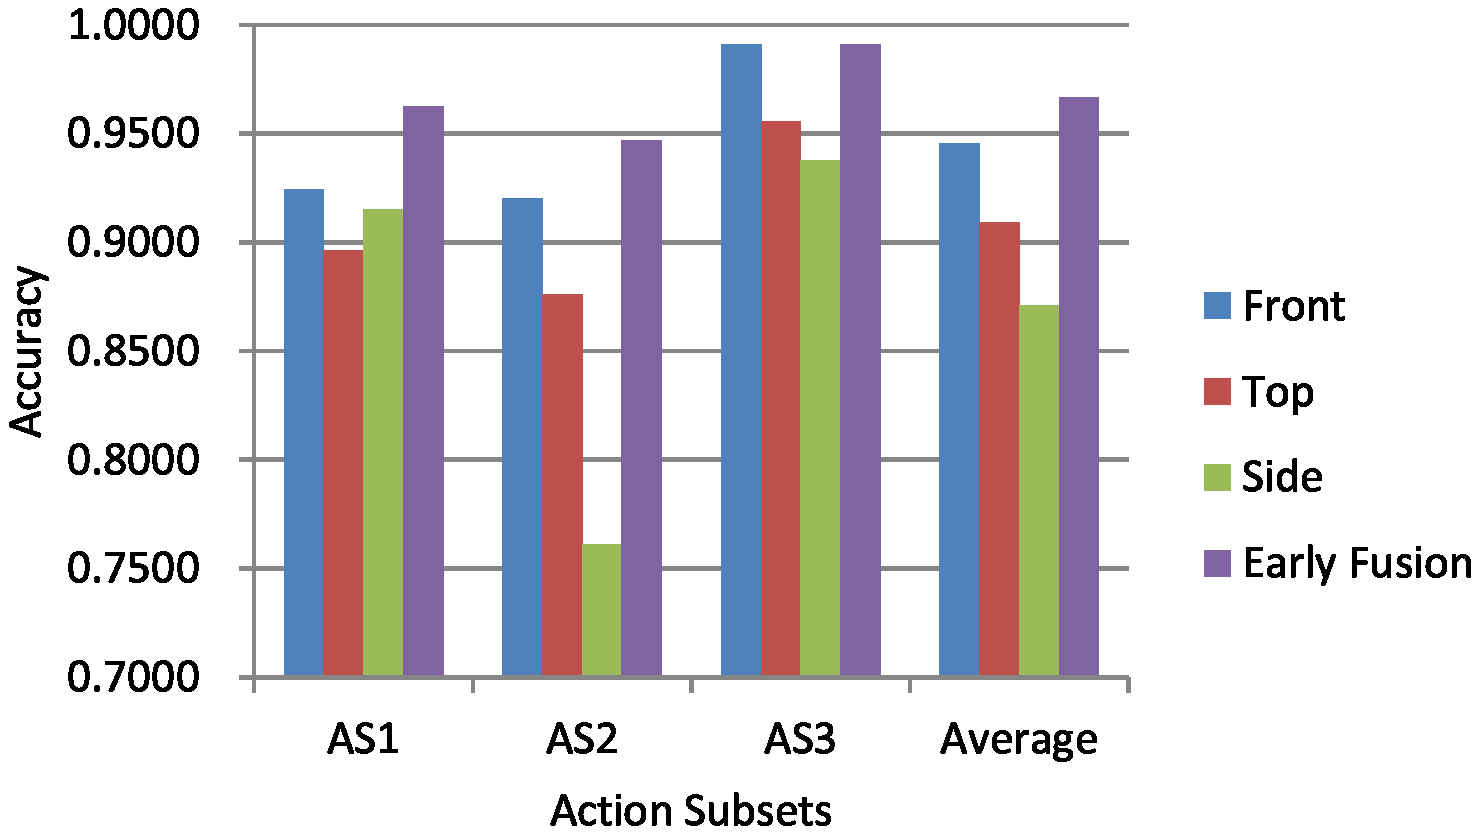
\includegraphics[scale=0.55]{Chart_EarlyFusion_AS123_MBH.eps}
	\end{center}
	\caption{\label{lbl:Figure_EarlyFusion_AS123_MBH}Results from using the early fusion scheme on representations}
\end{figure}
 
Beside, based on experimental results in figure \ref{lbl:Figure_EarlyFusion_AS123_MBH}, compensating information indicates two interesting points. The first one confirms that recognition result from front representation is better than the others (i.e. side and top). The second one shows that compensated information from other representations for front representation supports final predictions effectively. Thus, our proposed approach can be applied for any intensity-based techniques, in general.

\section{Discussions}
\label{lbl:Discussions}

\subsection{The Impact of Our Method on Descriptors}

For intensity data, according to \cite{wang2011densetraj} MBH is the best feature descriptor for dense trajectories. Therefore, in previous experiments, we only use MBH descriptor to represent motion information. Due to the difference between depth data and intensity data, how our approach has influenced other trajectory-aligned descriptors (i.e. HOG, HOF). In this section, we conduct similar experiments on these descriptors to answer this issue.

\begin{figure}[H]
	\begin{center}
		\includegraphics[scale=0.55]{Chart_ImpactOfDescriptors.eps}
	\end{center}
	\caption{\label{lbl:Figure_MBHHOGHOF}Results on trajectory-aligned descriptors}
\end{figure}

Figure \ref{lbl:Figure_MBHHOGHOF} shows interesting results. Although, recognition results on descriptors HOG, HOF are not good for each intensity representation, the final results after fusing have been significantly improved. The results indicate that the performances of HOG and HOF, respectively 94.53\% and 92.42\%, also outperform the state-of-the-art methods, as mentioned in Table \ref{lbl:Table_MBHvsSoAonFront}. In addition, lower-cost descriptors like HOG, HOF have more benefits for decreasing computational cost in processes, such as feature extraction and video representation (using the BoW model). These advantages provide a promising way for building effective and efficient systems.

\subsection{Evaluate the Role of Intensity Representations}

In this section, we consider the role of representations to our proposed method. Figure \ref{lbl:Figure_EarlyFusion_AS123_MBH} confirms that front representation achieves the best result. Obviously, it is an indispensable component to merge information. For the rest, we perform experiments on representation combinations with front representation. Experimental results are reported in Figure \ref{lbl:Figure_CombinationsFRONTSIDETOP}.

\begin{figure}[H]
	\begin{center}
		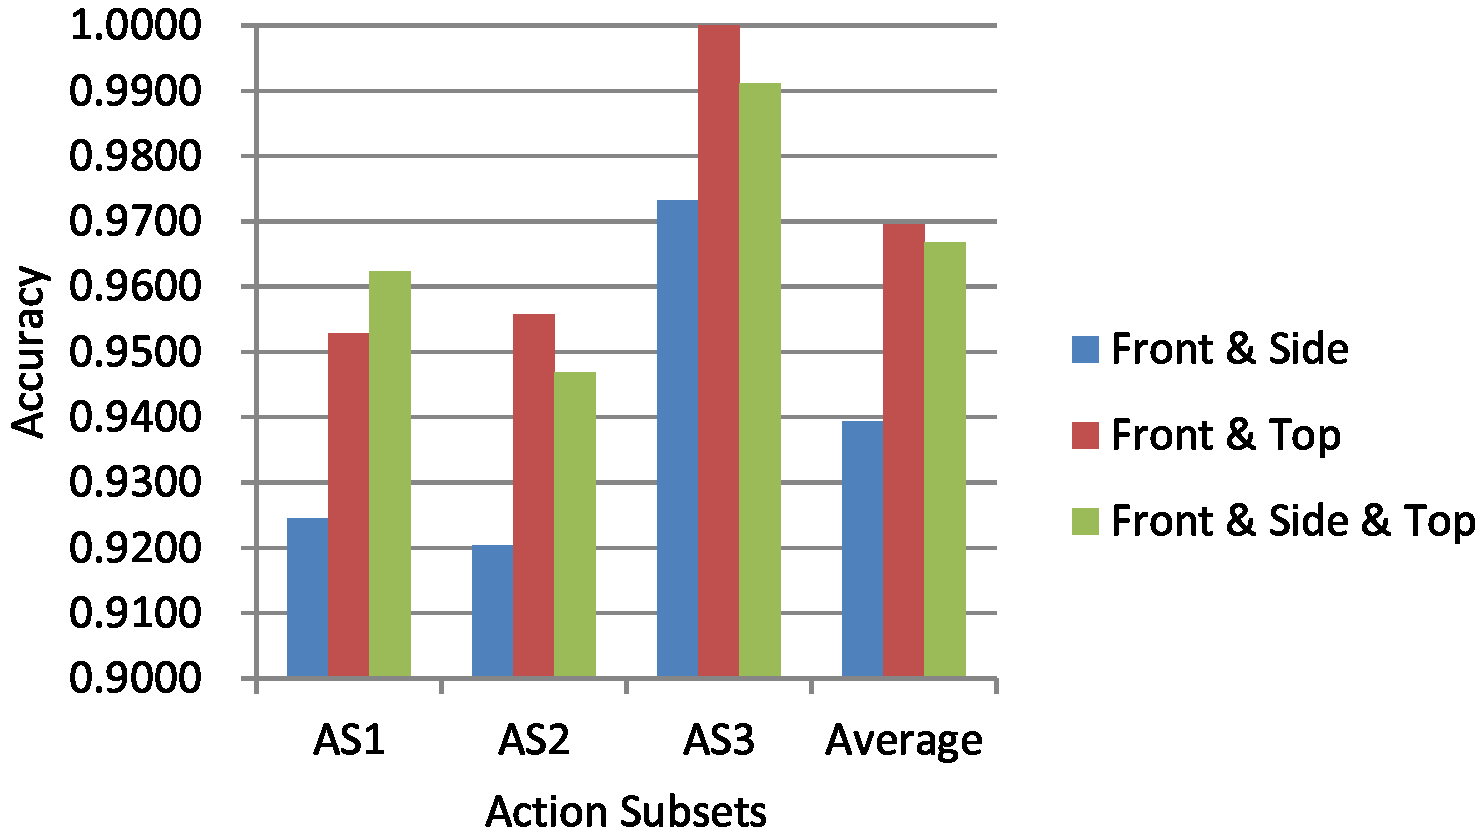
\includegraphics[scale=0.55]{Chart_RoleOfRepresentations.eps}
	\end{center}
	\caption{\label{lbl:Figure_CombinationsFRONTSIDETOP}Results on combinations of representations}
\end{figure}

In order to conduct the experiments, we create combinations: front and side, front and top. Figure \ref{lbl:Figure_CombinationsFRONTSIDETOP} indicates that the combination of front and top is better than the combination of front and side. More interestingly, the achieved performance, which is 96.95\% accuracy, from the combination of front and top beats the performance based on combining all the representations, in terms of average. Actually, the discovery provides a good choice to decrease computational cost but still ensures a convincing performance.

 \begin{table}[H]
 	\begin{center}
 		% Table generated by Excel2LaTeX from sheet 'Experiment-MSRDaily3D'
 		\begin{tabular}{c|c}
 		
 		{\bf Method} & {\bf Accuracy} \\
 		\hline
 		       LOP \cite{wang2012mining} &       42.5 \\
 		
 		     HON4D \cite{oreifej2013hon4d} &         52 \\
 		
 		DSTIP\&DCSF \cite{xia2013spatio} &      56.88 \\
 		\hline
 		{\bf Ours} & {\bf 62.5} \\
 		
 		\end{tabular}
 	\end{center}
 	\caption{\label{lbl:Table_Daily3D}Performance of Methods on MSR Daily Activity 3D Dataset. Notice that results are reported in terms of only using depth data.}
 \end{table}

\subsection{MSR Daily Activity 3D Dataset}

 The  MSR Daily Activity 3D dataset is proposed by \cite{wang2012mining}, which bao gồm 16 daily activities  (Fig. \ref{lbl:Figure_MSRDaily3D}) such as talking on the phone, reading a book, playing game, ... etc. In this dataset, background objects and subjects appear at different distances to the camera. Table \ref{lbl:Table_Daily3D} shows a comparison between the state-of-the-art methods on MSR Daily Activity 3D dataset. In this experiment, we conduct our trajectory-based approach only on front representation and use MBH descriptor to describe motion feature. In condition of only using depth data, \cite{wang2012mining, oreifej2013hon4d, xia2013spatio} report a unexpected performance. In \cite{xia2013spatio}, they modified this dataset to do evaluation. It is not fair to compare. Therefore, to ensure a fair comparison, we follow a framework similar to \cite{xia2013spatio} and evaluate on original MSR Daily Activity 3D dataset.
 
\begin{figure}[H]
%    \centering
    \subfloat[Reading book]{
        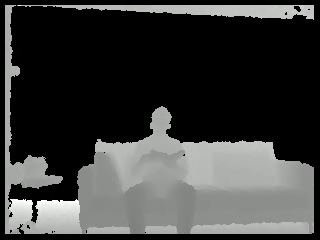
\includegraphics[width=0.45\textwidth]{ReadingBook.png}        
        }
    \hfill
    \subfloat[Drinking water]{
        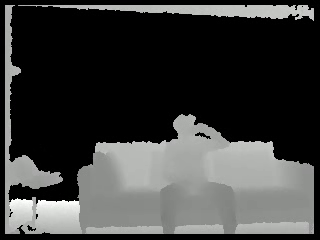
\includegraphics[width=0.45\textwidth]{DrinkingWater.png}        
        }
    \hfill
    \subfloat[Talking on a phone]{
        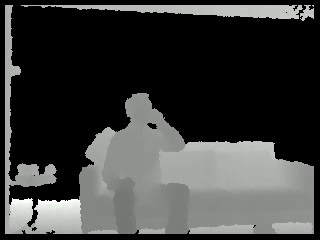
\includegraphics[width=0.45\textwidth]{TalkingOnAPhone.png}        
        }
    \hfill
    \subfloat[Playing game]{
        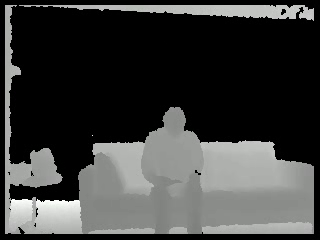
\includegraphics[width=0.45\textwidth]{PlayingGame.png}        
        }
    \hfill
    \subfloat[Writing on a paper]{
        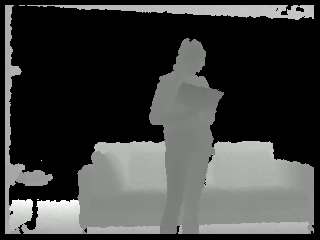
\includegraphics[width=0.45\textwidth]{WritingOnAPaper.png}        
        }
    \hfill
    \subfloat[Using a laptop]{
        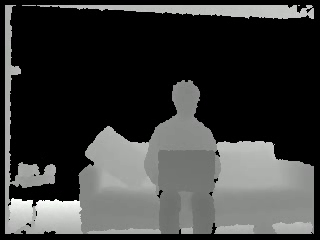
\includegraphics[width=0.45\textwidth]{UsingALaptop.png}        
        }
	\caption{\label{lbl:Figure_MSRDaily3D}Sample actions on MSR Daily Activity 3D dataset}
\end{figure}

Although our method outperforms all the state-of-the-art methods, it is not our aim. It is important to note that why in condition of only using depth data, most of methods are failed. When considering failed samples, such as \textit{playing a game}, \textit{writing on a paper}, and \textit{using a laptop}, we found that most of them are confused with action \textit{still}. For \textit{playing a game}, main action focus on motion of fingers, it is very difficult to discriminate from depth noise. For \textit{writing on a paper} and \textit{using a latop}, hand gestures are major actions to present motion information. But it is not fortunately, most of the movements are hidden by interactive objects (i.e. book, laptop). That is one reason to explain for the failure. The second one is performing similar movements with different objects, such as \textit{talking on the phone} and \textit{drinking water}. In these cases, objects is small and textureless. Thus it is very difficult to identify these actions exactly if only depending on depth data.

%\subsection{Early versus Late Fusion in Depth Motion Analysis}

%Liên quan đến vấn đề fusion, [snoek2005early] cung cấp một interesting work. Trong work này, tác giả đánh giá các semantic concepts trên 2 fusion schemes: early fusion và late fusion. Thí nghiệm được tiến hành trên the 2004 TRECVID benchmark dataset for visual modality and textual modality. Kết quả chỉ ra là late fusion scheme có khuynh hướng cho kết quả tốt hơn for most concepts. Đánh giá này cũng được sử dụng trong nhiều hệ thống dựa trên multimodal. Vậy đánh giá trên liệu có đúng cho cách tiếp cận của chúng tôi, khi xem xét mỗi intensity representation như là một modality. Để trả lời vấn đề này, chúng tôi thực hiện lại các thí nghiệm trên the late fusion scheme. Trong thí nghiệm này, chúng tôi sử dụng MBH descriptor để represent motion feature và tiến hành trên các tổ hợp representations: (front; side), (front; top) and (front; side; top). Kết quả thí nghiệm được chỉ ra ở Figure [EarlyLateFusion].

%Figure [EarlyLateFusion] cho thấy rằng cả hai the fusion schemes đều cho những significant improvements. Mặc dù vậy, do bởi các modalities có tính chất tương tự nhau (i.e. to represent motion information) nên 

\section{Conclusions}
\label{lbl:Conclusions}

We proposed using the trajectory-based approach for human action recognition using depth data in this work. We evaluated our approach by using the dense trajectories motion feature on MSR Action 3D datasets. More interestingly, our proposed trajectory-based approach only applied for one representation beats all the recent state-of-the-art approaches in terms of depth data. Beside, in order to deal with confused actions due to similar movements, compensating information from other representations is proposed. Therefore, the effectiveness of our approach on depth datasets like MSR is confirmed.

A trajectory-based approach with compensating information from separate representations shows promising results. This opens a general approach to leverage intensity-based techniques for depth data. This also suggests the importance of trajectory-based motion information on human action recognition using depth data. Therefore, exploiting depth-based motion trajectories can be beneficial for action recognition systems using depth cameras. This is also an interesting idea for our future work.

\section*{References}

\bibliographystyle{splncs}
\bibliography{JournalPaper_Ref}

\end{document}